Si vuole realizzare mediante Arduino un circuito che rilevi l’intensità della luce ambientale mediante un fotodiodo, e regoli la luce emessa da un LED di conseguenza. Si vuole che il LED sia spento/quasi spento in presenza di luce ambientale, e si accenda gradualmente fino al valore massimo al calare del livello di illuminazione sul fotodiodo. Sono stati utilizzati i seguenti componenti:
\begin{itemize}
    \item Resistenze $R_1$, $R_2$, $R_3$ da determinare, 0.25 W.
    \item LED 5 mm,  codice \textit{C503BRANCA0B0AA1}, Cree 
    \item Fotodiodo IR/visibile, codice \textit{P2N2222AG}, ON semiconductor
    \item Integrato operazionale a doppia uscita 6002, codice \textit{MCP 6002}
    \item Scheda Arduino DUE
\end{itemize}
Il circuito riportato in Figura \ref{fig:Circuit4} è alimentato mediante porta USB del PC, la quale eroga circa $(\sim 5 V)$. L'amplificatore operazionale richiederebbe alimentazione duale. Utilizziamo 0 V al terminale negativo per evitare errori che possano danneggiare la scheda Arduino.
\begin{figure}[H]
    \centering
    
\includegraphics[width=0.7\linewidth]{images/Circuit4.png}
    \caption{Schema circuito}
    \label{fig:Circuit4}
\end{figure}
La lettura del sensore di illuminazione, all'uscita dell'operazionale, viene fatta dal pin analogico \textbf{A0}, il LED è collegato al pin digitale \textbf{12}.
[FUNZIONAMENTO DEL CIRCUITO, $V_0$ vale...]
\clearpage
\subsection{Dimensionamento circuito e analisi}
Mediante il multimetro da banco è stata misurata la corrente generata dal fotodiodo in condizioni di illuminazione ambientale. 
\begin{equation*}
    I_{fotodiodo}= \text{ 1.1 } \mu\text{A}
\end{equation*}
Le resistenze sono state dimensionate in modo da ottenere
\begin{itemize}
    \item Tensione di uscita $V_0$ pari a circa 1 V (10\% errore max) in presenza di luce ambientale
    \item Corrente massima sul LED pari a 20 mA
\end{itemize}
Quindi sono state utilizzate le resistenze
\begin{equation*}
    R_1 = 1\text{ M}\Omega, R_2 = 1\text{ k}\Omega, R_3 = 68\text{ }\Omega
\end{equation*}
Dopo aver montato il circuito, si è usato l'oscilloscopio per misurare il valore di tensione di $V_0$ al variare del livello di illuminazione sul fotodiodo. Riportiamo in Figura \ref{fig:scope_0} la schermata dell'oscilloscopio
\begin{figure}[H]
    \centering
    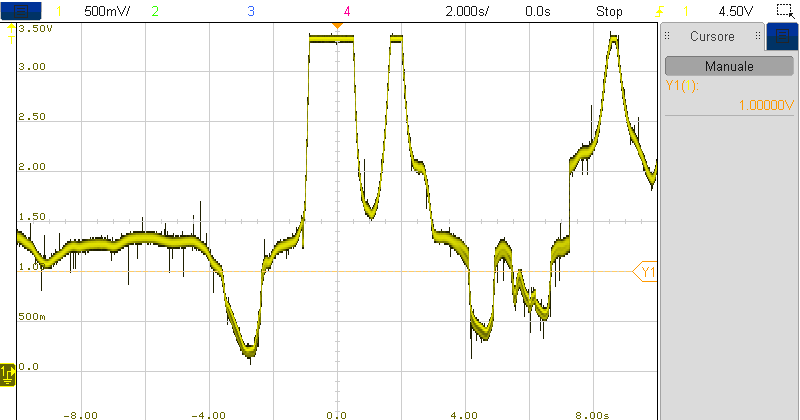
\includegraphics[width=\linewidth]{images/scope_0.png}
    \caption{Segnale di tensione $V_0$ al variare del livello di illuminazione sul fotodiodo}
    \label{fig:scope_0}
\end{figure}
E' possibile apprezzare il funzionamento del circuito dal video al \href{https://mediaspace.unipd.it/media/Esperimento+4/1_9r5biz93}{seguente link}
\subsubsection{Sensibilità alla luce ambientale artificiale}
Il sensore è sensibile all'oscillazione della luce ambientale (50Hz), infatti come vediamo in Figura \ref{fig:scope_1} andando ad analizzare l'uscita del circuito con l'oscilloscopio in accoppiamento AC notiamo che vi è la presenza di un oscillazione del segnale di uscita dal circuito a frequenze prossime ai 50 Hz.
\begin{figure}[H]
    \centering
    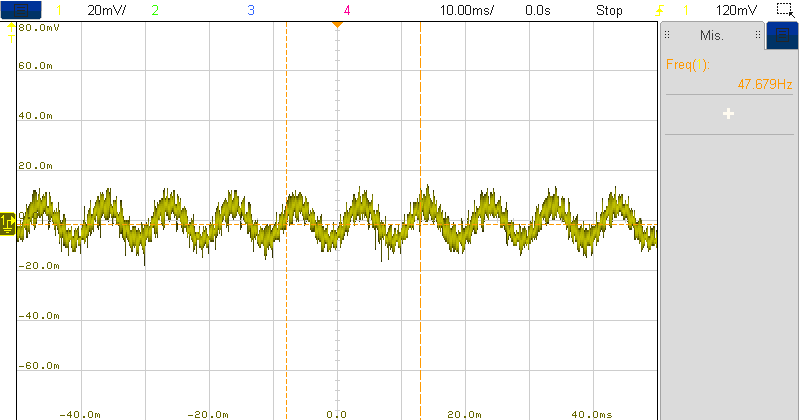
\includegraphics[width=\linewidth]{images/scope_1.png}
    \caption{Dettaglio in accoppiamento AC del segnale di tensione $V_0$}
    \label{fig:scope_1}
\end{figure}
Quindi si è deciso di stabilizzare il valore realizzando un filtro passa basso. Si è inserito un condensatore in parallelo a $R_1$ in modo da avere una frequenza di taglio di 10 Hz. 
\begin{equation}
    f_c=10 Hz \Longrightarrow C = 10nF
\end{equation}
Aggiungendo tale condensatore al circuito abbiamo notato che la componente di disturbo a 50 Hz è stata completamente smorzata, tuttavia il circuito per effetto dello stesso condensatore si è "rallentato", rispondendo meno istantaneamente alle variazioni di luminosità sul fotodiodo
\subsection{Codice}
\begin{lstlisting}[frame=single, language=Arduino]
const int ledPin =  12;     // the number of the LED pin
const int sensorPin = A0;   // the number of the light sensor pin

void setup(){
    pinMode(ledPin, OUTPUT);
}

void loop(){
    int sensorValue = analogRead(sensorPin);
    int light = map(sensorValue, 0, 1023, 255, 0);
    analogWrite(ledPin, light);
}
\end{lstlisting}